\documentclass[10pt]{article}

\usepackage{graphicx}
\usepackage{amsmath}
\usepackage{gensymb}
\usepackage{mathtools}
\usepackage{etoolbox}
\usepackage{booktabs}
\usepackage[parfill]{parskip}
\usepackage[numbers]{natbib}
\usepackage{float}
\usepackage{graphicx}
\usepackage{geometry}
\usepackage{multicol}
\usepackage{caption}

\newcommand\mgin{0.5in}
\geometry{
	left=\mgin,
	right=\mgin,
	bottom=\mgin,
	top=\mgin
}

% Set path to import figures from
\graphicspath{{../figures/}}

% Place converted graphics in current directory
\usepackage[outdir=./]{epstopdf}

% Define multicolumn figure-like environment
% from http://tex.stackexchange.com/questions/12262/multicol-and-figures
\newenvironment{mcfig}
	{\par\medskip\noindent\minipage{\linewidth}}
	{\endminipage\par\medskip}

% Define error function for math mode
\newcommand{\erf}{\mbox{erf}}
% Sign function
\newcommand{\sign}{\mbox{sign}}
% Natural numbers
\newcommand\N{\mathbb{N}}
% Real numbers
\newcommand\R{\mathbb{R}}
% Complex numbers
\newcommand\C{\mathbb{C}}
% Curly B for basis
\newcommand\BB{\mathcal{B}}
% Curly R for range (not real numbers)
\newcommand\RR{\mathcal{R}}
% Curly N for null space
\newcommand\NN{\mathcal{N}}
% Norm
\newcommand\norm[1]{\left\lVert #1 \right\rVert}
% Uniform Norm
\newcommand\unorm[1]{\left\lVert #1 \right\rVert_\infty}
% Inner Product
\newcommand\ip[1]{\left\langle #1 \right\rangle}
% Absolute value
\newcommand\abs[1]{\left| #1 \right|}
% Complex Conjugate
\newcommand\conj\overline
% Partial derivative
\newcommand\pd[2]{\frac{\partial #1}{\partial #2}}
% Disable paragraph indentation
\setlength{\parindent}{0pt}
% End of proof
\newcommand\qed{\hfill$\blacksquare$\hspace{0.5in}}

% Number this equation
\newcommand\eqnum{\addtocounter{equation}{1}\tag{\theequation}}

% arara: pdflatex
% arara: bibtex
% arara: pdflatex
% arara: pdflatex
\begin{document}

%%fakesection Title
\null

\thispagestyle{empty}
\addtocounter{page}{-1}

\begin{center}
    \begin{sffamily}
	\begin{bfseries}
	    \null
	    \vfill
		\Huge{Survey of Solution Techniques for Linear Systems from Finite Difference Methods in 2D Numerical Radiative Transfer}

	    \vspace{20pt}
	    \LARGE{Project Summary} \\
		\LARGE{ASSETs to Serve Humanity NSF REU 2016} \\
	    \vspace{20pt}
    \begin{Large}
		Oliver Evans \\
		Fred Weiss \\
		Christopher Parker \\
		Emmanuel Arkoh \\[1em]

		Dr. Malena Espa\~nol \\
	\vspace{20pt}
	\today
    \end{Large}
	\end{bfseries}
    \end{sffamily}
    \vspace{30pt}

    \null
    \vfill
    \vfill
    \null
\end{center}
\pagebreak


% Increase table cell height (not for header)
\renewcommand{\arraystretch}{1.5}

\begin{multicols}{2}

\section{Introduction}
We use monochromatic radiative transfer in order to model the light field in an aqueous environment populated by vegetation.
The vegetation (kelp) is modeled by a spatial probability distribution, which we assume to be given.
The two quantities we seek to compute are \textit{radiance} and \textit{irradiance}.
Radiance is the intensity of light in at a particular point in a particular direction, while irradiance is the total light intensity at a point in space, integrated over all angles.
The Radiative Transfer Equation is an integro-partial differential equation for radiance, which has been used primarily in stellar astrophysics; it's application to marine biology is fairly recent \citep{mobley_radiative_2001}.

We study various methods for solving the system of linear equations resulting from discretizing the Radiative Transfer Equation.
In particular, we consider direct methods, stationary iterative methods, and nonstationary iterative methods.
Numerical experiments are performed using Python's \texttt{scipy.sparse} \citep{jones_scipy:_2001} package for sparse linear algebra.
\texttt{IPython} \citep{perez_ipython:_2007} was used for interactive numerical experimentation.

Among those implemented, the nonstationary LGMRES \citep{baker_technique_2005} algorithm is the only algorithm determined to be suitable for this application without further work.
We discuss limitations and potential improvements, including preconditioning, alternative discretization, and reformulation of the RTE.

\subsection{Radiative Transfer}
Let $n$ be the number of spatial dimensions for the problem (i.e., 2 or 3).
Let $x \in \RR^n$.
Let $\Omega$ be the unit sphere in $\RR^n$.
Let $\omega \in \Omega$ be a unit vector in $\RR^n$.
Let $L(x,\omega)$ denote \textit{radiance} position $x$ in the direction $\omega$.
Let $I(x)$ denote \textit{irradiance} at position $x$.
Let $P_k(x)$ be the probability density of kelp at position $x$.
Let $a(x)$ and $b(x)$ denote the absorption and scattering coefficients respectively of the medium, which are both functions of $P_k$.
Let $\beta(\Delta\theta)$ denote the normalized \textit{volume scattering function} or \textit{phase function}, which defines the probability of light scattering at an angle $\Delta\theta$ from it's initial direction in a scattering event.

Then, the Monochromatic Radiative Transfer Equation (RTE) is
\begin{equation}
	\label{eq:rte}
	\begin{aligned}
		\omega \cdot \nabla_x L(x,\omega) &= -(a(x) + b(x)) L(x,\omega) \\
		&\qquad + b \int_\Omega \beta(\omega \cdot \omega') L(x,\omega')\, d\omega'
	\end{aligned}
\end{equation}

Note that in 2 spatial dimensions, this is a 3-dimensional problem ($x,y,\theta$).
Likewise, in 3 spatial dimensions, it is a 5-dimensional problem ($x,y,z,\theta,\phi$).

In this paper, we consider only the 2-dimensional problem, with the hope that sufficiently robust solution techniques for the 2-dimensional problem will be effective in the solution of the 3-dimensional problem, as well.

\subsection{2D Problem}
\label{sec:2d}
We use the downward-pointing coordinate system shown in figure \ref{fig:coords}, measuring $\theta \in [0,2\pi)$ from the positive $x$ axis towards the positive $y$ axis.
Further, we assume that the problem is given on the rescaled spatial domain $[0,1) \times [0,1)$, where $y=0$ is the air-water interface, and $y$ measures depth from the surface.

\begin{figure}[H]
	\centering
	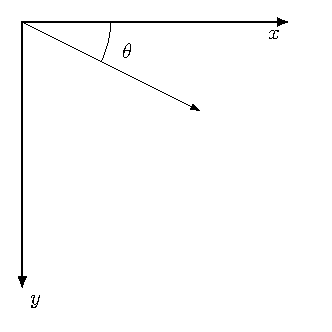
\includegraphics[width=2in]{2d_coords}
	\caption{2D coordinate system}
	\label{fig:coords}
\end{figure}

The 2-dimensional form of \eqref{eq:rte} is given by
\begin{equation}
	\begin{aligned}
		\pd{L}{x} \cos\theta + \pd{L}{y} \sin\theta
		&= -(a+b)L(x,y,\theta) \\
		&+ b\int_0^{2\pi} \beta(\abs{\theta-\theta'})\,d\theta',
	\end{aligned}
	\label{eq:rte2d}
\end{equation}

where $\abs{\theta-\theta'}$ measures the smallest angular difference between $]thet$ and $\theta'$ considering periodicity.

Note that in Cartesian coordinates, there are only spatial, not angular derivatives in the gradient.
In other coordinate systems, this is generally not the case.
	
\subsection{Boundary Conditions}
We assume that the downwelling light from the surface is known, and is defined to be uniform in space by the Dirichlet boundary condition 
\begin{equation}
	L(x,0,\theta) = f(\theta), \quad \mbox{for} \quad \theta \in [0,\pi).
	\label{eq:surf_bc}
\end{equation}

Note that we cannot apply the same idea to upwelling light at the surface, as it cannot be specified from information about the atmospheric light field.
Therefore, we apply the PDE at $y=0$ for $\theta \in [\pi,2\pi)$.

At $y=1$, we assume no upwelling light.
That is,
\begin{equation}
	L(x,0,\theta) = 0, \quad \mbox{for} \quad \theta \in [\pi,2\pi).
	\label{eq:bottom_bc}
\end{equation}

As with the upper $y$-boundary, we apply the PDE for $\theta \in [0,\pi)$ so as not to prohibit downwelling light.

In the horizontal direction, we assume periodic boundary conditions.
Assuming that a single discrete group of plants is being simulated, adjusting the width of the domain effectively modifies the spacing between adjacent groups of plants.

\section{Discretization}
In order to solve \eqref{eq:rte2d} numerically, we discretize the spatial derivatives using 2nd order central finite difference approximations (CD2), and we discretize the integral according to the Legendre-Gauss quadrature, as described in chapter 2 of \citet{chandrasekhar_radiative_1960}.
With this in mind, in order to create a spatial-angular grid with $n_x,n_y$, and $n_\theta$ discrete values for $x, y$, and $\theta$ respectively, we use a uniform square spatial discretization with spacing $dx, dy$, and a non-uniform angular discretization according to the roots of the Legendre Polynomial of degree $n_\theta$, denoted $P_{n_\theta}(\theta)$.
In each variable, we discard the uppermost grid point, as indicated by the half-open intervals in the previous sections.

Then, we have the grid
\begin{align}
	x_i &= i\,dx, &\quad i=1,\ldots,n_x \\
	y_j &= j\,dy, &\quad j=1,\ldots,n_y \\
	\theta_k \,\, \mbox{s.t.}\,\, 
	&P_{n_\theta}(\theta_k) = 0, &\quad k=1,\ldots,n_\theta
\end{align}

\subsection{Sparsity Plots}
\begin{figure}[H]
	\centering
	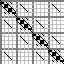
\includegraphics[width=3in]{../img/sparsity/int_small_4x4x4_012.png}
	\caption{Sparsity plot: 10x10x16, ordering 012}
\end{figure}

\begin{figure}[H]
	\centering
	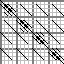
\includegraphics[width=3in]{../img/sparsity/int_small_4x4x4_210.png}
	\caption{Sparsity plot: 10x10x16, ordering 210}
\end{figure}
\subsection{Matrix Properties}
\subsubsection{Diagonal Dominance}
\subsubsection{Spectral Radius}

\section{Direct Methods}
\subsection{Factorizations}
\subsection{Software Packages}

\section{Stationary Iterative Methods}
\subsection{Fixed-Point Iteration}
\subsection{Convergence and Preconditioning}

\section{Nonstationary Iterative Methods}
\subsection{Krylov Subspace Methods}
\subsection{Convergence and Preconditioning}

\section{Numerical Results}

\section{Conclusions}

\nocite{*}
\bibliographystyle{abbrvnat}
\bibliography{rte_matrix_report}
\end{multicols}
>>>>>>> Stashed changes
\end{document}


